% !TEX TS-program = pdflatex
% !TEX encoding = UTF-8 Unicode

% Plantilla de la clase `scrartcl` del paquete KOMA-script
% Francisco Torralbo Torralbo
% 2019-03-04

\documentclass{scrartcl}

\KOMAoptions{%
  fontsize=12pt,      % Tamaño de fuente
  paper=a4,           % Tamaño del papel
  %titlepage=true,    % Reserva una página para el título.
  twoside=true,       % Para imprimir a doble página
  headings=normal,    % Tamaño de letra para los títulos: small, normal, big
  parskip=half,       % Espacio entre párrafos: full (una línea) o half (media línea)
  headsepline=false,  % Una linea separa la cabecera del texto
  %listof=totoc,      % Añadir a los contenidos la lista de tablas y figuras
  %bibliography=totoc,% Añadir a los contenidos una entrada para la bibliografía
  %bibliography=openstyle,  % oldstyle
}

% Personalización de la tipografía de diferentes elementos de página.
% En primer lugar definimos los colores que vamos a utilizar
\usepackage{color}
\definecolor{subject}{gray}{0.2} 
\definecolor{title}{RGB}{73, 35, 9} 
\definecolor{section}{RGB}{126, 64, 23}
\definecolor{subsection}{RGB}{190, 103, 45}

% A continuación definimos el tipo de letra, estilo y color de cada uno de los elementos que deseamos cambiar.
\setkomafont{titlehead}{\normalsize\itshape\color{subject}\centering}
\setkomafont{subject}{\large\scshape\color{subject}}
\setkomafont{title}{\color{title}}
\setkomafont{author}{\normalsize\bfseries}
\setkomafont{date}{\normalsize\sffamily}
\setkomafont{section}{\rmfamily\bfseries\color{section}}
\setkomafont{subsection}{\rmfamily\mdseries\color{subsection}}
\setkomafont{minisec}{\small\rmfamily\scshape\mdseries}
\setkomafont{caption}{\small\sffamily\color[gray]{0.3}}
\setkomafont{captionlabel}{\usekomafont{caption}}

\usepackage[activeacute,spanish]{babel}
\usepackage[utf8]{inputenc}
\selectlanguage{spanish}

\usepackage[T1]{fontenc}
\usepackage[sc,osf]{mathpazo}
\usepackage{tgpagella}
    \linespread{1} % Palatino needs more leading (space between lines)
%\usepackage[light,condensed,math]{iwona}
    \renewcommand{\sfdefault}{iwona}
\usepackage[toc,eqno,enum,bib,lineno]{tabfigures}
\usepackage[activate={true,nocompatibility},final,tracking=true,kerning=true,spacing=true,factor=1100,stretch=10,shrink=10]{microtype}

\usepackage{amsmath, amsfonts, amssymb}
\usepackage[mathscr]{eucal} % Proporciona el comando \mathscr para fuentes de tipo manuscrito en modo matemático sin sobreescribir el comando \mathcal

\usepackage{booktabs}
\renewcommand{\arraystretch}{1.5} % Aumenta el espacio vertical entre las filas de un entorno tabular

\usepackage{graphicx}
  % path to the graphics folder
  \graphicspath{{img/}}

\usepackage{hyperref}
\hypersetup{%
  % Descomentar la siguiente línea para crear enlaces con colores. 
  %colorlinks=true, linktocpage=true, pdfstartview=FitV,%
  %urlcolor=webbrown, linkcolor=RoyalBlue, citecolor=webgreen, %pagecolor=RoyalBlue,%
  % Descomentar la siguiente línea para crear enlaces en negro (útil para imprimir)
  colorlinks=false, linktocpage=false, pdfborder={0 0 0}, pdfstartpage=3, pdfstartview=FitV,% 
  pdftitle={Plantilla de la clase \texttt{scrartcl} del paquete KOMA-script},%
  pdfauthor={Francisco Torralbo},%
  pdfkeywords={LaTeX, curso, ugr, koma-script},%
  pdfcreator={pdfLaTeX},%
  pdfproducer={LaTeX with hyperref}%
}

\titlehead{Documento de ejemplo de personalización del paquete KOMA-Script}         
\subject{Curso latex}
\title{Personalizando una clase del paquete KOMA-Script}
\author{Francisco Torralbo Torralbo}

\begin{document}
\maketitle

\section{Introducción}
\begin{figure}
\centering
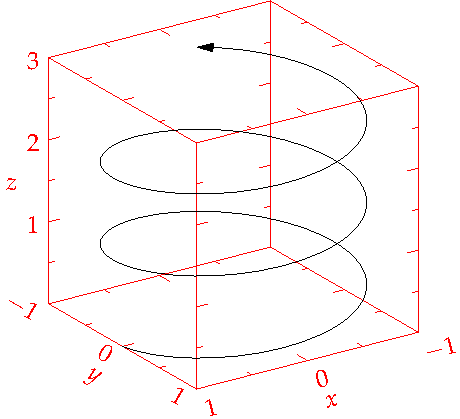
\includegraphics{helix.pdf}
\caption{Hélice}
\end{figure}

\subsection{Subsección de ejemplo}
\minisec{Mini sección de ejemplo}
Cada uno de los elementos de un documento: título, nombre del autor, seciones y capítulos, fecha, dedicatoria, citas, pies de página,\ldots tienen un tamaño y estilo de letra predefinido pero pueden cambiarse a voluntad. Para ello las clases del paquete KOMA-Script proporcionan dos comandos \verb+\setkomafont+ y \verb+\addtokomafont+ que permiten cambiar dicho estilo. En la documentación del paquete (ver pp. 60--63) podemos encontrar una lista completa de todos los elementos susceptibles de ser cambiados. Destacaremos aquí los más habituales:
\begin{description}
  \item[\texttt{title}] formato para el título (comando \verb+\title+)
  \item[\texttt{author}] formato para el nombre del autor (comando \verb+\author+) 
  \item[\texttt{titlehead}] formato para la cabecera sobre el título (comando \verb+\titlehead+)
  \item[\texttt{subject}] formato para el tema del documento (comando \verb+\subject+)
  \item[\texttt{date}] formato para la fecha (comando \verb+\date+)
  \item[\texttt{part}] formato para las partes del documento (comando \verb+\part+)
  \item[\texttt{chapter}] formato para los capítulos (comando \verb+\chapter+)
  \item[\texttt{chapterprefix}] formato para el texto ``Capítulo'' que suele anteponerse al nombre del capítulo 
  \item[\texttt{section}] formato para las secciones (comando \verb+\section+)
  \item[\texttt{subsection}] formato para las subseciones (comando \verb+\subsection+)
  \item[\texttt{minisec}] formato para las \emph{minisecciones} (comando \verb+\minisec+)
  \item[\texttt{dictum}] formato para las citas (comando \verb+\dictum+)
  \item[\texttt{caption}] formato para el título de una figura o tabla (comando \verb+\caption+) 
  \item[\texttt{captionlabel}] formato para la etiqueta del título de una figura o tabla (comando \verb+\caption+) 
  \item[\texttt{footnote}] formato para las notas al pie de página (comando \verb+\footnote+) 
  \item[\texttt{pagennumber}] formato para los números de página (comando \verb+\footnote+) 
\end{description}

These are usually commands like \verb+\rmfamily+, \verb+\sffamily+, \verb+\ttfamily+, \verb+\upshape+, \verb+\itshape+, \verb+\slshape+, \verb+\scshape+, \verb+\mdseries+, \verb+\bfseries+, \verb+\normalfont+, as well as the font size commands \verb+\Huge+, \verb+\huge+, \verb+\LARGE+, \verb+\Large+, \verb+\large+, \verb+\normalsize+, \verb+\small+, \verb+\footnotesize+, \verb+\scriptsize+, and \verb+\tiny+
% \verb+\usefontofkomafont{element}+ \verb+\usesizeofkomafont{element}+

Este documento ha cambiado varias de dichas opciones para definir un estilo propio.

\end{document}
